\documentclass[a4paper,12pt]{book} \usepackage[utf8]{inputenc} \title{} \author{Rachel Morris} \date{\today}

\usepackage{rachwidgets}
\usepackage{fancyhdr} \usepackage{lastpage} \usepackage{dirtree} \usepackage{boxedminipage} \usepackage{tikz}  \usepackage{circuitikz}
\usepackage{colortbl} % cell bg colors

\newcommand{\laClass}{CS 210\ } \newcommand{\laSemester}{Fall 2017\ }
\newcommand{\laChapter}{Chapter 3\ } \newcommand{\laExam}{Exam 3\ }

%\toggletrue{answerkey}
\togglefalse{answerkey}

\newcounter{question}
\newcounter{answer}

\newtoggle{testingCenter}
\togglefalse{testingCenter}

\pagestyle{fancy}
\fancyhf{}
\lhead{\laClass}
\chead{\laSemester}
\rhead{Exam 3 preview}
\rfoot{\thepage\ of \pageref{LastPage}}
\lfoot{\scriptsize By Rachel Morris, last updated \today}

\renewcommand{\headrulewidth}{2pt}
\renewcommand{\footrulewidth}{1pt}

\begin{document}

    \section*{\laExam, \laChapter preview}

    \laClass \laSemester{}

    \subsection*{Chapter 3.1: Set definitions and operations}

%----------------------------------------------------------------------%
\stepcounter{question}
    \paragraph{Question \thequestion} ~\\
        Using these sets:

        \begin{center}
            \begin{tabular}{p{6cm} p{4cm} p{4cm} }
                $U = \{ 1, 2, 3, 4, 5, 6, 7, 8, 9, 10 \}$
                & $A = \{ 5, 6, 9 \}$
                & $B = \{ 3, 4, 9, 10 \}$
                \\
                & $C = \{ 5, 6 \}$
                & $D = \{ 2, 6, 8 \}$
            \end{tabular}
        \end{center}

        Find the results of the following set operations:

            ~\\
            a.   $A - C$        \tab
            b.   $C - A$        \tab
            c.   $A \cap C$     \\
            d.   $A \cup D$     \tab
            e.   $A'$           \tab[1.7cm]
            f.   $C \cup B$

%----------------------------------------------------------------------%
\stepcounter{question}
    \paragraph{Question \thequestion} ~\\

        Fill in the Venn diagrams for each of the following statements.
        Remember to include the Universe.
        ~\\

        \begin{tabular}{p{4cm} p{4cm} p{4cm}}
            a. $U - A$ &
            b. $B' - A$ &
            c. $A \cup (B - C)$
            \\
            \venndiagram & \venndiagram & \venndiagram
        \end{tabular}

%----------------------------------------------------------------------%
\stepcounter{question}
    \paragraph{Question \thequestion} ~\\

        Write the following in set-builder notation with the form description:

        \begin{enumerate}
            \item[a.]   The set of odd integers.
            \item[b.]   The set of natural numbers that are even.
        \end{enumerate}


    \subsection*{Chapter 3.2: More operations on sets}

%----------------------------------------------------------------------%
\stepcounter{question}
    \paragraph{Question \thequestion} ~\\

        Using these sets:

            \begin{center}
                $A = \{ fast, slow \}$ \tab $B = \{ bike, car \}$
            \end{center}

        Find the result of the following:

        \begin{enumerate}
            \item[a.]   $A \times B = $
            \item[b.]   $\wp(B) = $
            \item[c.]   List out all 2 partitions of $A$.
        \end{enumerate}

%----------------------------------------------------------------------%
\stepcounter{question}
    \paragraph{Question \thequestion} ~\\

Using these sets:

            \begin{center}
                $A = \{ 1, 2 \}$ \tab $B = \{ a, b \}$
            \end{center}

        Find the result of the following:

        \begin{enumerate}
            \item[a.]   $A \times B = $
            \item[b.]   $\wp( A \times B ) = $
            \item[c.]   $\wp(A) = $
            \item[d.]   $\wp(B) = $
            \item[e.]   Fill out the table for $\wp(A) \times \wp(B)$ :

                \begin{tabular}{ c | p{2.5cm} | p{2.5cm} | p{2.5cm} | p{2.5cm} }
                    & $\emptyset$ & $\{1\}$ & $\{2\}$ & $\{1, 2\}$
                    \\ \hline
                    $\emptyset$ & & & &
                    \\ \hline
                    $\{a)$ & & & &
                    \\ \hline
                    $(b)$ & & & &
                    \\ \hline
                    $(a, b)$ & & & &
                    \\
                \end{tabular}

                Write out the set $\wp(A) \times \wp(B) = $
        \end{enumerate}



    \subsection*{Chapter 3.4: Boolean algebra}

%----------------------------------------------------------------------%
\stepcounter{question}
    \paragraph{Question \thequestion} ~\\

        Rewrite each of the following with the equivalent Boolean Algebra version.
        Convert upper-case Set names to lower-case variables $(A \to a)$ but
        keep the same letters for propositional variables $(p \to p)$.

            ~\\
            a. $(A \cup B)$     \tab
            b. $C - D$          \tab
            c. $p \land q$      \\
            d. $\neg q$         \tab[1.8cm] 
            e. $(A \cap B)'$    \tab[0.6cm]
            f. $\neg(p)$



\subsection*{Chapter 3.5: Logic circuits}

%----------------------------------------------------------------------%
\stepcounter{question}
    \paragraph{Question \thequestion} ~\\

        Identify the Boolean Expression for the following diagrams.
        You \underline{do not} need to simplify it.

        \begin{enumerate}
            \item[a.] ~\\

                \begin{circuitikz}
                    % Frame
                    \draw (-2,-1) -- (5,-1) -- (5,2) -- (-2,2) -- (-2,-1);

                    % Gates
                    \draw   (1,1.3)       node[american and port] {};
                    \draw   (3,1)       node[american or port] {};

                    % Line
                    \draw (1,1.3) -- (2,1.3);
                    \draw (-0.5, -0.5) -- (1,-0.5) -- (1.6,0.7);

                    % Labels
                    \node [fill=none] at (-1,1.3) (nodeS) {a};
                    \node [fill=none] at (-1,0.7) (nodeS) {b};
                    \node [fill=none] at (-1,-0.5) (nodeS) {c};
                \end{circuitikz}

                \solution{ $(a \cdot b) + c$ }{}

            \item[b.] ~\\

                \begin{circuitikz}
                    % Frame
                    \draw (-2,1) -- (5,1) -- (5,4) -- (-2,4) -- (-2,1);

                    % Gates
                    \draw   (4,3)       node[american or port] {};
                    \draw   (1,2)       node[american not port] {};

                    \draw   (-0.5,2) -- (0.5,2);
                    \draw   (1.7,2) -- (2.6,2.72);
                    \draw   (-0.5,3.3) -- (2.6, 3.28);

                    % Labels
                    \node [fill=none] at (-1,3.3) (nodeS) {a};
                    \node [fill=none] at (-1,2) (nodeS) {b};
                \end{circuitikz}

                \solution{ $ (a + b') $ }{}
        \end{enumerate}

%----------------------------------------------------------------------%
\stepcounter{question}
    \paragraph{Question \thequestion} ~\\

    Draw a circuit diagram for the following Boolean Expression:

    $$ a'b + b'c $$



%----------------------------------------------------------------------%
\stepcounter{question}
    \paragraph{Question \thequestion} ~\\

        For the following Karnaugh map:

        \begin{center}
            \begin{tabular}{c c c}
                & $y$ & $y'$ \\ \cline{2-3}
                $x$     & \multicolumn{1}{|c}{  } & \multicolumn{1}{|c|}{ \checkmark } \\ \cline{2-3}
                $x'$    & \multicolumn{1}{|c}{ \checkmark } & \multicolumn{1}{|c|}{ \checkmark } \\ \cline{2-3}
            \end{tabular}
        \end{center}

        Identify the following:

        \begin{enumerate}
            \item[a.]   All 3 terms:
            \item[b.]   Simplified equation:
        \end{enumerate}

%----------------------------------------------------------------------%
\stepcounter{question}
    \paragraph{Question \thequestion} ~\\

        Simplify the following Boolean Expression. Mark the terms in the
        Karnaugh map, then build out rectangles to come up with a simplified expression.

        $$ xyz' + xy'z' + x'yz + x'yz' + x'y'z' + x'y'z $$

        \begin{center}
            \begin{tabular}{c c c c c}
                & $yz$ & $yz'$ & $y'z'$ & $y'z$ \\ \cline{2-5}
                $x$     & \multicolumn{1}{|c }{  }
                        & \multicolumn{1}{|c }{  }
                        & \multicolumn{1}{|c }{  }
                        & \multicolumn{1}{|c|}{  } \\ \cline{2-5}
                $x'$    & \multicolumn{1}{|c }{  }
                        & \multicolumn{1}{|c }{  }
                        & \multicolumn{1}{|c }{  }
                        & \multicolumn{1}{|c|}{  } \\ \cline{2-5}
            \end{tabular}
        \end{center}

\hrulefill

% #################################################################### %

\toggletrue{answerkey}
%\togglefalse{answerkey}

    \section*{\laExam, \laChapter preview answer key}

    \subsection*{Chapter 3.1: Set definitions and operations}

%----------------------------------------------------------------------%
\stepcounter{answer}
    \paragraph{Question \theanswer}

    ~\\
    1.   $A - C$  = \solution{ $ \{ 9 \} $ }{} \tab
    2.   $C - A$ = \solution{ $ \emptyset $ }{} \tab
    3.   $A \cap C$ = \solution{ $\{ 5, 6 \}$ }{} \tab{}

    ~\\
    4.   $A \cup D$ = \solution{ $ \{ 2, 5, 6, 8, 9 \} $ }{} \tab
    5.   $A'$ = \solution{ $ \{ 1, 2, 3, 4, 7, 8, 10 \} $ }{} \tab{}

    ~\\
    6.   $C \cup B$ = \solution{ $ \{ 3, 4, 5, 6, 9, 10 \} $ }{} \tab

%----------------------------------------------------------------------%
\stepcounter{answer}
    \paragraph{Question \theanswer} ~\\

        \begin{tabular}{p{4cm} p{4cm} p{4cm}}
            a. $U - A$ &
            b. $B' - A$ &
            c. $A \cup (B - C)$
            \\

            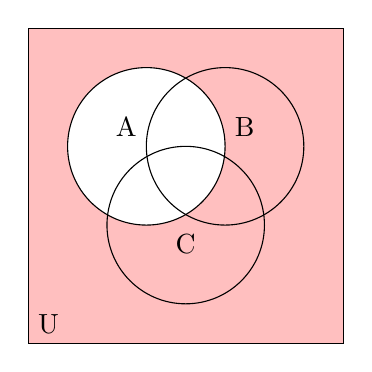
\begin{tikzpicture}[even odd rule]
                \scope
                    \clip (1.5, 2.5) circle (1cm) (0,0) rectangle (4,4);
                    \fill[pink] (0, 0) rectangle (4, 4);
                \endscope
                \draw (0,0) -- (4,0) -- (4,4) -- (0,4) -- (0,0) node[anchor=south west] {U};
                \draw (1.5, 2.5) circle (1cm) node[anchor=south east] {A};
                \draw (2.5, 2.5) circle (1cm) node[anchor=south west] {B};
                \draw (2, 1.5) circle (1cm) node[below] {C};
            \end{tikzpicture}
            &
            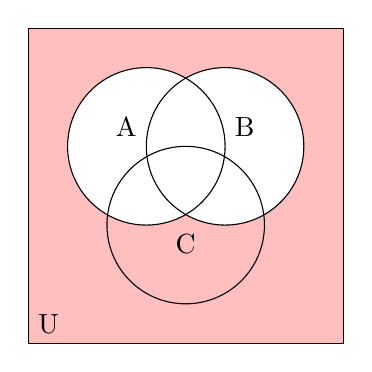
\begin{tikzpicture}[even odd rule]
                \scope
                    \clip (1.5, 2.5) circle (1cm) (0,0) rectangle (4,4);
                    \clip (2.5, 2.5) circle (1cm) (0,0) rectangle (4,4);
                    \fill[pink] (0, 0) rectangle (4, 4);
                \endscope
                \draw (0,0) -- (4,0) -- (4,4) -- (0,4) -- (0,0) node[anchor=south west] {U};
                \draw (1.5, 2.5) circle (1cm) node[anchor=south east] {A};
                \draw (2.5, 2.5) circle (1cm) node[anchor=south west] {B};
                \draw (2, 1.5) circle (1cm) node[below] {C};
            \end{tikzpicture}
            &
            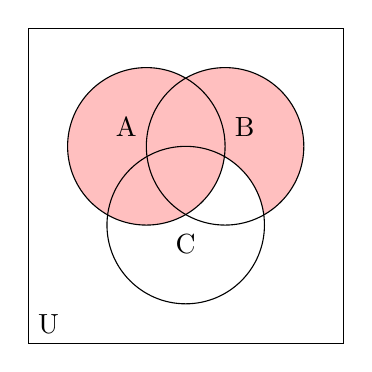
\begin{tikzpicture}[even odd rule]
                \scope
                    \fill[pink] (1.5,2.5) circle (1cm);
                    \clip (2, 1.5) circle (1cm) (0,0) rectangle (4,4);
                    \fill[pink] (2.5,2.5) circle (1cm);
                \endscope
                \draw (0,0) -- (4,0) -- (4,4) -- (0,4) -- (0,0) node[anchor=south west] {U};
                \draw (1.5, 2.5) circle (1cm) node[anchor=south east] {A};
                \draw (2.5, 2.5) circle (1cm) node[anchor=south west] {B};
                \draw (2, 1.5) circle (1cm) node[below] {C};
            \end{tikzpicture}
        \end{tabular}
        
%----------------------------------------------------------------------%
\stepcounter{answer}
    \paragraph{Question \theanswer} ~\\

        \begin{enumerate}
            \item[a.]   The set of odd integers.
                \solution{ $\{ 2k+1 : k \in \mathbb{Z} \}$ }{}
            \item[b.]   The set of natural numbers that are even.
                \solution{ $\{ 2k : k \in \mathbb{N} \}$ }{}
        \end{enumerate}

%----------------------------------------------------------------------%
\stepcounter{answer}
    \paragraph{Question \theanswer} ~\\

        \begin{enumerate}
            \item[a.]   $A \times B = $
                \solution{ $\{ (fast, bike), (fast, car), (slow, bike), (slow, car) \}$ }{}

            \item[b.]   $\wp(B) = $
                \solution{ $\{ \emptyset, \{bike\}, \{car\}, \{bike, car\} \}$ }{}

            \item[c.]   List out all 2 partitions of $A$.
                \solution{
                    \begin{enumerate}
                        \item   $\{ \{fast\}, \{slow\} \}$
                        \item   $\{ \{fast, slow\} \}$
                    \end{enumerate}
                }{}
        \end{enumerate}

%----------------------------------------------------------------------%
\stepcounter{answer}
    \paragraph{Question \theanswer} ~\\

        \begin{enumerate}
            \item[a.]   $A \times B = $
                \solution{ $\{ (1, a), (1, b), (2, a), (2, b) \}$ }{ }
            \item[b.]   $\wp( A \times B ) = $
                \solution{
                    $\{
                        \emptyset, \\
                        \{ (1, a) \}, \{ (1, b) \}, \{ (2, a) \}, \{ (2, b) \}, \\
                        \{ (1, a), (1, b) \}, \{ (1, a), (2, a) \}, \{ (1, a), (2, b) \}, \\
                        \{ (1, b), (2, a) \}, \{ (1, b), (2, b) \}, \{ (2, a), (2, b) \}, \\
                        \{ (1, a), (1, b), (2, a) \}, \{ (1, a), (1, b), (2, b) \}, \\
                        \{ (1, a), (2, a), (2, b) \}, \{ (1, b), (2, a), (2, b) \}, \\
                        \{ (1, a), (1, b), (2, a), (2, b) \}
                    \}$
                }{ }
            \item[c.]   $\wp(A) = $
                \solution{ $\{ \emptyset, \{1\}, \{2\}, \{1,2\} \}$ }{  }
            \item[d.]   $\wp(B) = $
                \solution{ $\{ \emptyset, \{a\}, \{b\}, \{a, b\} \}$ }{ }
            \item[e.]   Fill out the table for $\wp(A) \times \wp(B)$ :

                THESE ARE BACKWARDS * NEED TO FIX.

                \begin{tabular}{ c | p{2.5cm} | p{2.5cm} | p{2.5cm} | p{2.5cm} }
                    & $\emptyset$ & $\{1\}$ & $\{2\}$ & $\{1, 2\}$
                    \\ \hline
                    $\emptyset$
                        & \solution{ $( \emptyset, \emptyset )$ }{}
                        & \solution{ $( \emptyset, \{1\} )$ }{}
                        & \solution{ $( \emptyset, \{2\} )$ }{}
                        & \solution{ $( \emptyset, \{1, 2\} )$ }{}
                    \\ \hline
                    $\{a)$
                        & \solution{ $( \{a\}, \emptyset )$ }{}
                        & \solution{ $( \{a\}, \{1\} )$ }{}
                        & \solution{ $( \{a\}, \{2\} )$ }{}
                        & \solution{ $( \{a\}, \{1, 2\} )$ }{}
                    \\ \hline
                    $(b)$
                        & \solution{ $( \{b\}, \emptyset )$ }{}
                        & \solution{ $( \{b\}, \{1\} )$ }{}
                        & \solution{ $( \{b\}, \{2\} )$ }{}
                        & \solution{ $( \{b\}, \{1, 2\} )$ }{}
                    \\ \hline
                    $(a, b)$
                        & \solution{ $( \{a, b\}, \emptyset )$ }{}
                        & \solution{ $( \{a, b\}, \{1\} )$ }{}
                        & \solution{ $( \{a, b\}, \{2\} )$ }{}
                        & \solution{ $( \{a, b\}, \{1, 2\} )$ }{}
                    \\
                \end{tabular}

                Write out the set $\wp(A) \times \wp(B) = $
                \solution{ $\{
                    ( \emptyset, \emptyset ),  ( \emptyset, \{1\} ),
                    ( \emptyset, \{2\} ), ( \emptyset, \{1, 2\} ), \\
                    ( \{a\}, \emptyset ), ( \{a\}, \{1\} ), ( \{a\}, \{2\} ), ( \{a\}, \{1, 2\} ) \\
                    ( \{b\}, \emptyset ), ( \{b\}, \{1\} ), ( \{b\}, \{2\} ), ( \{b\}, \{1, 2\} ) \\
                    ( \{a, b\}, \emptyset ), ( \{a, b\}, \{1\} ), ( \{a, b\}, \{2\} ), ( \{a, b\}, \{1, 2\} )
                \}$ }{  }
        \end{enumerate}

%----------------------------------------------------------------------%
\stepcounter{answer}
    \paragraph{Question \theanswer}

        ~\\
        $(A \cup B)$                \solution{ $(a + b)$ }{ \vspace{1cm} }      \tab[2cm]
        $C - D$                     \solution{ $c \cdot d'$ }{ \vspace{1cm} }   \\
        $p \land q$                 \solution{ $p \cdot q$ }{ \vspace{1cm} }    \tab[3cm]
        $\neg q$                    \solution{ $q'$ }{ \vspace{1cm} }           \\
        $(A \cap B)'$               \solution{ $(a \cdot b)'$ }{ \vspace{1cm} } \tab[2cm]
        $\neg(p)$                   \solution{ $(p)'$ }{ \vspace{1cm} }


%----------------------------------------------------------------------%
\stepcounter{answer}
    \paragraph{Question \theanswer} ~\\

        \begin{enumerate}
            \item[a.]
                \solution{ $(a \cdot b) + c$ }{}

            \item[b.]
                \solution{ $ (a + b') $ }{}
        \end{enumerate}

\newpage
%----------------------------------------------------------------------%
\stepcounter{answer}
    \paragraph{Question \theanswer} ~\\

    \solution{
    \begin{circuitikz}
        % Frame
        \draw (-2,0) -- (10,0) -- (10,4) -- (-2,4) -- (-2,0);

        % Gates
        \draw   (3,1)    node[american and port] {};
        \draw   (3,3)    node[american and port] {};

        \draw   (1,1.28)    node[american not port] {};
        \draw   (1,3.28)    node[american not port] {};

        \draw   (6,2)    node[american or port] {};

        \draw   (-0.5, 3) -- (0,3) -- (0, 3.3) -- (0.5, 3.3);
        \draw   (-0.5, 1) -- (0,1) -- (0, 0.5) -- (1.6, 0.5) -- (1.6, 0.7);

        \draw   (-0.5, 2) -- (0,2) -- (0,1.3) -- (0.5, 1.3);
        \draw                (0,2) -- (1.0,2) -- (1.0, 2.7) -- (1.6, 2.7);

        \draw   (3,1) -- (4,1) -- (4,1.72) -- (4.7, 1.72);
        \draw   (3,3) -- (4,3) -- (4, 2.28) -- (4.7, 2.28);

        % Labels
        \node [fill=none] at (-1,3) (nodeS) {a};
        \node [fill=none] at (-1,2) (nodeS) {b};
        \node [fill=none] at (-1,1) (nodeS) {c};
    \end{circuitikz}
    }{}

%----------------------------------------------------------------------%
\stepcounter{answer}
    \paragraph{Question \theanswer} ~\\

        \begin{enumerate}
            \item[a.]   All 3 terms:            \solution{ $x'y$, $x'y'$, $xy'$ }{}
            \item[b.]   Simplified equation:    \solution{ $x' + y'$ }{}
        \end{enumerate}

%----------------------------------------------------------------------%
\stepcounter{answer}
    \paragraph{Question \theanswer} ~\\

        \begin{center}
            \begin{tabular}{c c c c c}
                & $yz$ & $yz'$ & $y'z'$ & $y'z$ \\ \cline{2-5}
                $x$     & \multicolumn{1}{|c }{  }
                        & \multicolumn{1}{|c }{ \cellcolor{blue!25}\checkmark }
                        & \multicolumn{1}{|c }{ \cellcolor{blue!25}\checkmark }
                        & \multicolumn{1}{|c|}{  } \\ \cline{2-5}
                $x'$    & \multicolumn{1}{|c }{ \cellcolor{red!25}\checkmark }
                        & \multicolumn{1}{|c }{ \cellcolor{purple!25}\checkmark }
                        & \multicolumn{1}{|c }{ \cellcolor{purple!25}\checkmark }
                        & \multicolumn{1}{|c|}{ \cellcolor{red!25}\checkmark } \\ \cline{2-5}
            \end{tabular}
        \end{center}

        Can simplify to...
        $$ x' + z' $$

\end{document}
